\documentclass{article}
\usepackage[utf8]{inputenc}
\usepackage[margin = 0.8in]{geometry}
\usepackage{graphicx}
\usepackage{amsmath, amssymb}
\usepackage{subcaption}
\usepackage{multirow}
\usepackage{mathtools}
\usepackage{float}
\usepackage{pythonhighlight}

\title{RBE549 - Homework 12}
\author{Keith Chester}
\date{Due date: December 13th, 2022}

\begin{document}
\maketitle

\section*{Problem 1}
In stero imaging, if the rays define by $\vec{X}_L$ and $\vec{X}_R$ do not intersect, we can find $\vec{X}_W$ anyway by minimizing an error measure. One way to do this is to project $\vec{X}_W$ into the left and the right image planes to give $\vec{X}_L'$ and $\vec{X}_R'$. The error $E$ is defined as the squared difference between the observed image points $\vec{X}_L$ $\vec{X}_R$ and the projected points $\vec{X}_L'$ and $\vec{X}_R'$.

\subsection*{A}

In this problem, we are asked to show that for the simplified parallel optical axis camera geometry used in class where $\vec{f} \cdot \vec{B} = 0, R=I,\vec{T}=\pm\frac{\vec{B}}{2}$.

\noindent We accomplish this by starting with the given definition of error:

\begin{equation}
    E = |\vec{X}_L'-\vec{X}_L|^2 + |\vec{X}_R' - \vec{X}_R|^2
\end{equation}

\noindent ...which we can expand the definition to mean literally:

\begin{equation}
    E = (x_L' - x_L)^2 + (y_L' - y_L)^2 + (z_L' - z_L)^2 + (x_R' - x_R)^2 + (y_R' - y_R)^2 + (z_R' - z_R)^2
\end{equation}

\noindent Since we know that $X_L'$ and $X_R'$ are projections we can use the imaging equation with an offset for the camera from $x_W$ by $\frac{\pm b}{2}$.

\begin{equation}
    x_R'=\frac{f}{z_W}\bigl( x^W - \frac{b}{2} \bigr)
\end{equation}

\begin{equation}
    y_R' = \frac{f}{z_W}\bigl( y^W \bigr)
\end{equation}

\begin{equation}
    x_L'=\frac{f}{z_W}\bigl( x^W + \frac{b}{2} \bigr)
\end{equation}

\begin{equation}
    y_L' = \frac{f}{z_w}\bigl( y^W \bigr)
\end{equation}

\noindent ...this allows us to do some introductions:

\begin{equation}
    E = (\frac{f}{z^W}\bigl( x^W + \frac{b}{2} \bigr) - x_L)^2 + (\frac{f}{z^W}\bigl( y^W \bigr) - y_L)^2 + (z_L' - z_L)^2 + ( x_R'=\frac{f}{z^W}\bigl( x^W - \frac{b}{2} \bigr) - x_R)^2 + (\frac{f}{z^W}\bigl( y^W \bigr) - y_R)^2 + (z_R' - z_R)^2
\end{equation}

\noindent ...and we can note that $z_L'=z_L$ and $z_R'=z_R$:

\begin{equation}
    E = (\frac{f}{z^W}\bigl( x^W + \frac{b}{2} \bigr) - x_L)^2 + (\frac{f}{z^W}\bigl( y^W \bigr) - y_L)^2 + ( x_R'=\frac{f}{z^W}\bigl( x^W - \frac{b}{2} \bigr) - x_R)^2 + (\frac{f}{z^W}\bigl( y^W \bigr) - y_R)^2
\end{equation}

\subsection*{B}

In this problem, we are asked to show that, by differentiating $E$ with respect to $x^W$ and $y^W$, to show that:

\begin{equation}
    x^W = \frac{x_L + x_R}{2} \frac{z^W}{f},y^W=\frac{y_l+  y_R}{2}\frac{z^W}{f}
\end{equation}

\noindent To do this, we take the partial derivative $\frac{\partial}{\partial x^W} E$ and $\frac{\partial}{\partial y^W} E$:

\begin{equation}
    \frac{\partial}{\partial x^W} E = 
    \frac{2f}{z^W} \bigl(\frac{f}{z^W} (x^W+\frac{b}{2})-x_L\bigr) + 
    \frac{2f}{z^W} \bigl(\frac{f}{z^W} (x^W-\frac{b}{2})-x_R\bigr)
\end{equation}

\begin{equation}
    \frac{\partial}{\partial x^W} E = \frac{2f}{z^W}\bigl( 
        \frac{2}{z^W}x^W-x_L-x_R
    \bigr)
\end{equation}

\noindent...We can do a similar approach for our $\frac{\partial}{\partial y^W} E$:

\begin{equation}
    \frac{\partial}{\partial x^W} E = 
    \frac{2f}{z^W} \bigl(\frac{f}{z^W} (y^W+\frac{b}{2})-y_L\bigr) + 
    \frac{2f}{z^W} \bigl(\frac{f}{z^W} (y^W-\frac{b}{2})-y_R\bigr)
\end{equation}

\begin{equation}
    \frac{\partial}{\partial y^W} E = \frac{2f}{z^W}\bigl( 
        \frac{2}{z^W}y^W-y_L-y_R
    \bigr)
\end{equation}

\noindent Since these are errors, we set them to 0 for minimizing:

\begin{equation}
    0 = \frac{2f}{z^W}\bigl( 
        \frac{2}{z^W}x^W-x_L-x_R
    \bigr)
\end{equation}

\begin{equation}
    0 = \frac{2}{z^W}x^W-x_L-x_R
\end{equation}

\begin{equation}
    \frac{2}{z^W}x^W = x_L+x_R
\end{equation}

\begin{equation}
    \frac{x_L+x_R}{2}\frac{z^W}{f}=x^W
\end{equation}

\noindent ...and similarly, we'd fine for $y^W$:

\begin{equation}
    \frac{y_L+y_R}{2}\frac{z^W}{f}=y^W
\end{equation}

\subsection*{C}

In this problem, we are asked to show that

\begin{equation}
    z^W = \frac{fb}{\Delta x}
\end{equation}

\noindent ...concluding that

\begin{equation}
    \vec{X}^W=\vec{X}_{AVG}\frac{|\vec{B}|^2}{\vec{B}\vec{\Delta}}
\end{equation}

\noindent We begin by looking at our function $E$ again:

\begin{equation}
    E = (\frac{f}{z^W}\bigl( x^W + \frac{b}{2} \bigr) - x_L)^2 + (\frac{f}{z^W}\bigl( y^W \bigr) - y_L)^2 + ( x_R'=\frac{f}{z^W}\bigl( x^W - \frac{b}{2} \bigr) - x_R)^2 + (\frac{f}{z^W}\bigl( y^W \bigr) - y_R)^2
\end{equation}

\noindent ...and then take the partial derivative $\frac{\partial}{\partial z^W} E$:

\begin{equation}
    \frac{\partial}{\partial z^W} E = 
    \frac{2f}{z^w}
    \bigl(
        \frac{f}{z^W}(x^W+\frac{b}{2})-x_L
    \bigr)\bigl( x^W + \frac{b}{2} \bigr) + 
    \frac{2f}{z^w} \bigl( \frac{f}{z^W} y^W -y_L \bigr) y^W +
    \frac{2f}{z^w} \bigl(\frac{f}{z^W}(x^W - \frac{b}{2}-x_R) \bigr)\bigl(x^W-\frac{b}{2}\bigr) +
    \frac{2f}{z^w} \bigl(y^W - y_R \bigr)y^W
\end{equation}

\begin{equation}
    \begin{split}
    \frac{\partial}{\partial z^W} E = \frac{2f}{z^w}\biggl(
        \bigl((\frac{f}{z^w}x^W+\frac{f}{z^w}\frac{b}{2})-x_L\bigr)\bigl(x^W+\frac{b}{2}\bigr)+
        \bigl((\frac{f}{z^w}y^W)-y_L\bigr)y^W + \\
        \bigl((\frac{f}{z^w}x^W-\frac{f}{z^w}\frac{b}{2})-x_R\bigr)\bigl(x^W-\frac{b}{2}\bigr)+
        \bigl((\frac{f}{z^w}y^W-\frac{f}{z^w}\frac{b}{2})-y_R\bigr)\bigl(y^W\bigr)
    \biggr)
    \end{split}
\end{equation}

\begin{equation}
    \begin{split}
    \frac{2f}{z^w}\biggl(
        \bigl(\frac{f}{z^w}x^{W^2}+\frac{f}{z^w}\frac{b}{2}x^W-x_Lx^W\bigr)+
        \bigl(\frac{b}{2}\frac{f}{z^w}x^W+\frac{f}{z^w}\frac{b^2}{4}-\frac{b}{2}x_L\bigr) +
        \bigl(\frac{f}{z^w}y^{W^2}+\frac{f}{z^w}\frac{b}{2}y^W-y_Ly^W\bigr)+ \\
        \bigl(\frac{f}{z^w}X^{W^2}-\frac{f}{z^w}\frac{b}{2}x^W-x^Wx_R\bigr) +
        \bigl(-\frac{f}{z^w}\frac{b}{2} x^W + \frac{f}{z^w} \frac{b^2}{4}+\frac{b}{2}x_R\bigr)
        \bigl(\frac{f}{z^w}y^{W^2}-\frac{f}{z^w}\frac{b}{2}y^W-y_Ry^W\bigr)
    \biggr)
    \end{split}
\end{equation}

\noindent We can then gather like terms, factor out  $\frac{2f}{z^W}$, and set to 0:

\begin{equation}
    0 = \frac{2f}{z^W} \bigl(x^{W^2}+y^{W^2}\bigr)-x^W(x_L+x_R)-y^W(y_L+y_R)+\frac{fb^2}{2z^W} + \frac{x_Rb}{2}-\frac{x_Lb}{2}
\end{equation}

\noindent ...if you recall, we can use our equation replacements from part B here:

\begin{equation}
    \begin{split}
    0 = \frac{2f}{z^W} \biggl(
        \bigl(\frac{x_L+x_R}{2}\frac{z^W}{f}\bigr) + 
        \bigl(\frac{y_L+y_R}{2}\frac{z^W}{f}\bigr) -
        \bigl(\frac{x_L+x_R}{2}\frac{z^W}{f}\bigr)(x_L+x_R) -\\
        \bigl(\frac{y_L+y_R}{2}\frac{z^W}{f}\bigr)(y_L+y_R)+
        \frac{fb^2}{2z^W} + \frac{x_Rb}{2}-\frac{x_Lb}{2}
    \biggr)
    \end{split}
\end{equation}

\noindent We can simplify, due to massive cancellations, to:

\begin{equation}
    0 = \frac{fb^2}{2z^W} + \frac{x_Rb}{2}-\frac{x_Lb}{2}
\end{equation}

\begin{equation}
    \frac{fb}{z^W}=x_L-x_R
\end{equation}

\begin{equation}
    z^W = \frac{fb}{x_L-x_R}
\end{equation}

\noindent We can define $\Delta x = x_L-x_R$:

\begin{equation}
    z^W = \frac{fb}{\Delta x}
\end{equation}

\noindent We can then plug into our definitions from above:

\begin{equation}
    \vec{X}^W = \begin{bmatrix}
        \frac{x_L+x_R}{2}\frac{z^W}{f} \\
        \frac{y_L+y_R}{2}\frac{z^W}{f} \\
        \frac{fb}{\Delta x}
    \end{bmatrix}
\end{equation}

\noindent We can pull out the $\frac{z^W}{f}$:

\begin{equation}
    \vec{X}^W = \frac{z^W}{f}\begin{bmatrix}
        \frac{x_L+x_R}{2} \\
        \frac{y_L+y_R}{2} \\
        \frac{fb}{\Delta x} \frac{f}{z^W}
    \end{bmatrix}
\end{equation}

\noindent As we stated before, $f = \frac{z_L+z_R}{2}$, so:

\begin{equation}
    \vec{X}^W = \frac{fb}{\frac{\Delta x}{f}}\begin{bmatrix}
        \frac{x_L+x_R}{2} \\
        \frac{y_L+y_R}{2} \\
        \frac{z_L+z_R}{2}
    \end{bmatrix}
\end{equation}

\noindent ...which can be expressed as what we set out to show:

\begin{equation}
    \begin{bmatrix}
        x^W \\ y^W \\ z^W
    \end{bmatrix} = \vec{X}_{AVG} \frac{|\vec{B}|^2}{B\Delta x}
\end{equation}

\section{Problem 2}

Another way to determine distance when $\vec{X}_L$ and $\vec{X}_R$ do not intersect is to find the point $\vec{X}^W$ closest to the rays $\vec{X}_L$ and $\vec{X}_R$. Here we define the left image ray as:

\begin{equation}
    \vec{X}_L^W = -\frac{\vec{B}}{2}+l\vec{X}_L,0\leq l
\end{equation}

\noindent ...and the right image ray as:

\begin{equation}
    \vec{X}_R^W = \frac{\vec{B}}{2}+r\vec{X}_R,0\leq r
\end{equation}

\begin{figure}[H]
    \centering
    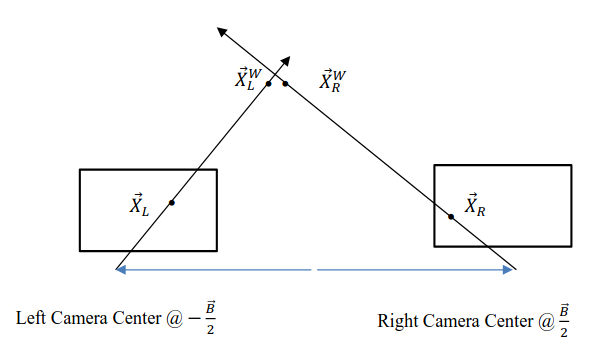
\includegraphics[width = 0.75\textwidth]{imgs/problem_2.png}
    \caption{Problem 2}
    \label{fig:prob-2}
\end{figure}

The goal is to find points $X_L^W$ and $X_R^W$ on the left and right image rays that are closest to each other; the point equidistant between them is the desired $\vec{X}^W$. We can find these points by minimizing:

\begin{equation}
    min_{l,r}|\vec{X}_L^W-\vec{X}_L^W|
\end{equation}

\noindent ...show that the solution is given by:

\begin{equation}
    \vec{X}^W=\frac{1}{2}\frac{\bigl(
        |\vec{X}_R|^2(\vec{X}_L\vec{B})-(\vec{X}_L\vec{X}_R)(\vec{X}_R\vec{B})\bigr)\vec{X}_L
        +
        \bigl(
            (\vec{X}_L\vec{X}_R)(\vec{X}_L\vec{B})-|\vec{X}_L|^2(\vec{X}_R\vec{B})
        \bigr)\vec{X}_R}{|\vec{X}_L|^2|\vec{X}_R|^2 - (\vec{X}_L\vec{X}_R)^w}
\end{equation}

\noindent To approach this, we will start by taking the $\partial l$ and $\partial r$, then set it equal to $0$. Starting with $|X_L^W-X_R^W|^2$, we can subsibtute:

\begin{equation}
    |(\frac{-\vec{B}}{2}+l\vec{X}_L)-(\frac{\vec{B}}{2}+r\vec{X}_R)|^2
\end{equation}

\begin{equation}
    \bigl(-\frac{\vec{B}}{2} +l\vec{X}_L\bigr)^2-
    2\bigl(-\frac{\vec{B}}{2}+l\vec{X}_L\bigr)
    \bigl(\frac{\vec{B}}{2}+r\vec{X}_R\bigr) +
    \bigl(\frac{\vec{B}}{2}+r\vec{X}_R\bigr)^2
\end{equation}

\noindent We can fenagle this with algebra to get:

\begin{equation}
    \begin{split}
        \frac{|\vec{B}|^2}{2} - \vec{B}l\vec{X}_L + l^2|\vec{X}_L|^2+\frac{2|\vec{B}|^2}{4} - l\vec{X}_L\vec{B}+\vec{B}r\vec{X}_R \\
        - 2l\vec{X}_Lr\vec{X}_R+\frac{|\vec{B}|^2}{4}+\vec{B}r\vec{X}_R+r^2|\vec{X}_R|^2
    \end{split}
\end{equation}

\begin{equation}
    |\vec{B}|^2-2\vec{B}\vec{X}_L+l^2|\vec{X}_L|^2-2l(\vec{X}_L\vec{X}_R)+2r(\vec{B}\vec{X}_R)+r^2|\vec{X}_R|^2
\end{equation}

\noindent Now we take $\partial l$ of above:

\begin{equation}
    0 = -2\vec{B}\vec{X}_L+2l|\vec{X}_L|^2-2r\vec{X}_L\vec{X}_R
\end{equation}

\noindent Now we solve for $r$:

\begin{equation}
    r = \frac{2\vec{B}\vec{X}_L-2l|\vec{X}_L|^2}{-2\vec{X}_L\vec{X}_R}
\end{equation}

\noindent We can now subsibtute to solve:

\begin{equation}
    \frac{2\vec{B}\vec{X}_L-2l|\vec{X}_L|^2}{-2\vec{X}_L\vec{X}_R} = \frac{2l\vec{X}_L\vec{X}_R-2\vec{B}\vec{X}_r}{2|\vec{X}_R|^2}
\end{equation}

\noindent Solving for l in MATLAB:

\begin{equation}
    l = \frac{\bigl(|\vec{X}_R|^2(\vec{B}\cdot\vec{X}_L)-(\vec{X}_L\cdot\vec{X}_R)(\vec{B}\cdot\vec{X}_r)\bigr)}{|\vec{X}_R|^2|\vec{X}_L|^2-(\vec{X}_L\cdot\vec{X}_R)^2}
\end{equation}

\begin{equation}
    l = \frac{2(\vec{X}_R\cdot\vec{B})+2r|\vec{X}_R|^2}{2(\vec{X}_L\cdot\vec{X}_R)}
\end{equation}

\noindent and having MATLAB solve for $r$:

\begin{equation}
    r = \frac{(\vec{X}_L\cdot\vec{X}_R)(\vec{X}_L\vec{B})-|\vec{X}_L|^2(\vec{X}_R\cdot\vec{B})}{|\vec{X}_L|^2|\vec{X}_R|^2-(\vec{X}_L\cdot\vec{X}_R)^2}
\end{equation}

\noindent We can then subsibtute this back into our equations for $\vec{X}^W_{L/R}$:

\begin{equation}
    \vec{X}_R^W = \frac{B}{2} + \frac{(\vec{X}_L\cdot\vec{X}_R)(\vec{X}_L\vec{B})-|\vec{X}_L|^2(\vec{X}_R\cdot\vec{B})}{|\vec{X}_L|^2|\vec{X}_R|^2-(\vec{X}_L\cdot\vec{X}_R)^2} \vec{X}_R
\end{equation}

\begin{equation}
    \vec{X}_L^W = -\frac{B}{2} + \frac{(\vec{X}_L\cdot\vec{X}_R)(\vec{X}_L\vec{B})-|\vec{X}_L|^2(\vec{X}_R\cdot\vec{B})}{|\vec{X}_L|^2|\vec{X}_R|^2-(\vec{X}_L\cdot\vec{X}_R)^2} \vec{X}_L
\end{equation}

\noindent Since we're looking for the midway point, it'd be defined as $\frac{1}{2}$ between these:

\begin{equation}
    \frac{1}{2}\biggl(
        -\frac{B}{2} + \frac{(\vec{X}_L\cdot\vec{X}_R)(\vec{X}_L\vec{B})-|\vec{X}_L|^2(\vec{X}_R\cdot\vec{B})}{|\vec{X}_L|^2|\vec{X}_R|^2-(\vec{X}_L\cdot\vec{X}_R)^2} \vec{X}_L + \frac{B}{2} + \frac{(\vec{X}_L\cdot\vec{X}_R)(\vec{X}_L\vec{B})-|\vec{X}_L|^2(\vec{X}_R\cdot\vec{B})}{|\vec{X}_L|^2|\vec{X}_R|^2-(\vec{X}_L\cdot\vec{X}_R)^2} \vec{X}_R
    \biggr)
\end{equation}

\noindent ...and our $\frac{\pm\vec{B}}{2}$ cancels:

\begin{equation}
    \frac{1}{2}\biggl(
        \frac{(\vec{X}_L\cdot\vec{X}_R)(\vec{X}_L\vec{B})-|\vec{X}_L|^2(\vec{X}_R\cdot\vec{B})}{|\vec{X}_L|^2|\vec{X}_R|^2-(\vec{X}_L\cdot\vec{X}_R)^2} \vec{X}_L + \frac{(\vec{X}_L\cdot\vec{X}_R)(\vec{X}_L\vec{B})-|\vec{X}_L|^2(\vec{X}_R\cdot\vec{B})}{|\vec{X}_L|^2|\vec{X}_R|^2-(\vec{X}_L\cdot\vec{X}_R)^2} \vec{X}_R
    \biggr)
\end{equation}

\noindent ...which is what we sought to find!


\end{document}